\chapter{Architecture}
\label{chap:archimpl}
 
In this chapter is discussed the architecture of the solution that we
implemented. We decided to design a two-layer MANO architecture that will manage
the service function chains. Along with the architecture is described how it
will be deployed on Kubernetes.

\section{Overview}
\begin{figure}[H]
  \centering
  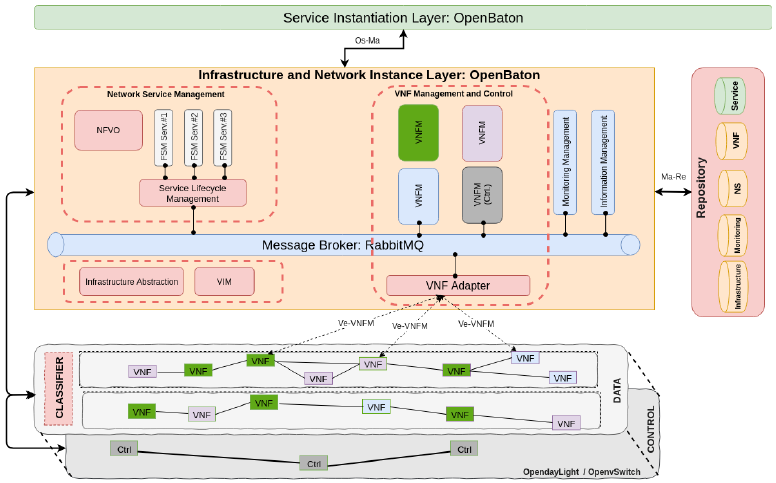
\includegraphics[scale=0.5]{Architecture}
  \caption{Architecture of a two-layer orchestration framework}
  \label{chap:archimpl:img:architecture}
\end{figure}
In Figure~\ref{chap:archimpl:img:architecture} is depicted the overall
architecture of the expected implementation. All components communicate each
other thanks to RabbitMQ and the system is orchestrated by Openbaton. Unlike the
ETSI NFV framework the technologies involved are defined, and this was the
system proposal to which we started. The low-level orchestration handles
repositories for VNFs and SFCs definitions, monitoring and service deployment.

The higher level, instead, instructs the lower one through the APIs that it
exposes, configuring and managing services. 

We study this architectural proposal and the technologies proposed but we had
some troubles with some of the components. In fact, we choose to deploy our
platform on Kubernetes but we were not able to make Openbaton and this container
orchestrator work together.

Openbaton has a plugin structure that allows developer to integrate new
features. We tried to developed an Openbaton VIM driver to allow this MANO to
deploy functions and chains on Kubernetes, but it requires to manage their
definitions using TOSCA. This standard language for describe cloud based
services topology focus on hypervisor virtualization and its resource usage.
This was an issue to our problem in which we have to exploit containers.

\section{Our proposal}
After evaluating technologies and the starting architecture, we decide to
implement our management and orchestration solution, to be integrated with
Kubernetes and container technologies, \texttt{Harbor}. It manages data
repositories for VNFs and SFCs definition as well as their lifecycle.
\texttt{Harbor} was implemented to expose a RESTful API that allow managing
component deployed in a Openbaton-like manner. 

\begin{figure}[H]
  \centering
  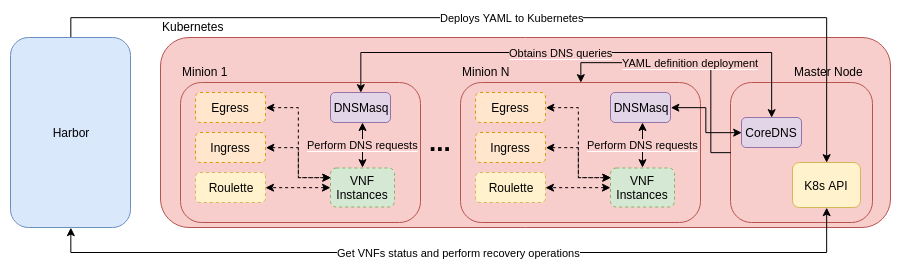
\includegraphics[scale=0.5]{architectureproposal}
  \caption{Final architecture}
  \label{chap:archimple:sec:secondattempt:img:attempt2v1harbor}
\end{figure}

To describe SFC \texttt{Harbor} uses a JSON definition, for VNF, instead, it
requires a YAML definition, as the one used by Kubernetes. 

Thanks to the APIs, it is possible to integrate our system with Openbaton: in
fact it is possible to create a plugin and map it call to \texttt{Harbor} ones.
In order to fully support this tool the real effort will be to provide the
possibility to deploy chains and virtual functions on Kubernetes. 

To Kubernetes is demanded the management of the connectivity among the
components of the platform and the handling of the virtualized resources.
Nodes on Kubernetes are divided in master and slaves: the former gives access to
Kubernetes APIs, allowing for example to launch containers on the cluster, and
orchestrate other nodes, instead the latter elements, also called
\emph{Minions}, are the nodes on which Pods are deployed.

Kubernetes default installation is comprehensive of a DNS, \emph{CoreDNS}, for
name resolution. In order to reduce the number of requests to the DNS on each
Minion is deployed a Dnsmasq instance, that is a local DNS cache that cooperate
with CoreDNS.